\documentclass{article}

\usepackage[a4paper,top=2cm,bottom=2cm,left=3cm,right=3cm,marginparwidth=1.75cm]{geometry}


\usepackage{amsmath}
\usepackage{graphicx}
\usepackage[colorlinks=true, allcolors=blue]{hyperref}
\usepackage{subcaption} % Required for subtable environment
\usepackage{booktabs}
\usepackage{multirow}

\usepackage{listings}
\renewcommand{\lstlistingname}{Wykaz}

\usepackage{float}



\usepackage[dvipsnames,svgnames,x11names,table]{xcolor}

\definecolor{vertexStart}{RGB}{44, 160, 44} 
\definecolor{vertexEnd}{RGB}{214, 39, 40} 
\definecolor{vertexConnect}{RGB}{31, 119, 180}
\definecolor{vertexDivide}{RGB}{255, 127, 14}
\definecolor{vertexRegular}{RGB}{148, 103, 189}

\lstdefinestyle{mystyle}{
    backgroundcolor=\color{backcolour},   
    commentstyle=\color{codegreen},
    keywordstyle=\color{magenta},
    numberstyle=\tiny\color{gray},
    stringstyle=\color{codepurple},
    basicstyle=\ttfamily\footnotesize,
    breakatwhitespace=false,         
    breaklines=true,                 
    captionpos=b,                    
    keepspaces=true,                 
    numbers=left,                    
    numbersep=5pt,                  
    showspaces=false,                
    showstringspaces=false,
    showtabs=false,                  
    tabsize=2
}

\lstset{style=mystyle}
\lstset{language=Python}

% Define colors
\definecolor{backcolour}{rgb}{0.95,0.95,0.92}
\definecolor{codegreen}{rgb}{0,0.6,0}
\definecolor{codepurple}{rgb}{0.58,0,0.82}
\definecolor{magenta}{rgb}{0.5,0,0}

\usepackage[polish]{babel}
\usepackage[utf8]{inputenc} % Added for proper Polish character support
\usepackage[T1]{fontenc}    % Added for better font encoding

% --- fancyhdr Package and Setup ---
\usepackage{fancyhdr}
\pagestyle{fancy}
\fancyhf{} % Clear all header and footer fields
\renewcommand{\headrulewidth}{0.4pt} % Add a rule under the header

\lhead{Ivan Lazorenko, Bartłomiej Wiśniewski}
\rhead{Algorytmy macierzowe, ćwiczenie 1}
\cfoot{Strona \thepage}
% --- End of fancyhdr Setup ---

% 1. Load biblatex and specify 'biber' as the backend
\usepackage[backend=biber, style=numeric]{biblatex}

% 2. Point to your .bib file (include the extension .bib!)
\addbibresource{sample.bib}

\title{Algorytmy macierzowe, ćwiczenie 1}
\author{Ivan Lazorenko, Bartłomiej Wiśniewski}

\newcommand{\BigO}[1]{\mathcal{O}(#1)}

\begin{document}


\maketitle
\thispagestyle{empty} % This command removes the header and footer from the title page


\section{Dane techniczne}

Do wszystkich obliczeń wykorzystuję następujące parametry:

\begin{enumerate}
    \item komputer MacBook Pro M4, architektura procesora ARM; 16 GB pamięci operacyjnej, 
    \item interaktywnego notatnika \texttt{Jupyter Notebook}, korzystając z wersji \texttt{Python 3.12.6}.
\end{enumerate}

\section{Rekurencyjne mnożenie macierzy}

Tematem sprawozdania jest analiza rekurencyjnych algorytmów mnożenia macierzy postaci $C = A \cdot B$. Do podstawowych algorytmów z tej grupy należy metoda Bineta (klasyczne mnożenie blokowe), opierająca się na strategii ,,dziel i zwyciężaj''. Metoda ta pozwala na wyznaczanie iloczynu poprzez rekurencyjny podział macierzy wejściowych na mniejsze bloki.

Na początku rozważymy mechanizm działania algorytmu Bineta. Dla macierzy $A$ i $B$ o wymiarach $n \times n$ (w przypadku parzystego $n$), macierze wejściowe dzielone są na cztery submacierze o wymiarach $\frac{n}{2} \times \frac{n}{2}$:

\[
A = \begin{pmatrix} 
A_{11} & A_{12} \\ 
A_{21} & A_{22} 
\end{pmatrix}, \quad
B = \begin{pmatrix} 
B_{11} & B_{12} \\ 
B_{21} & B_{22} 
\end{pmatrix}
\]

Zauważmy, że macierz wynikowa $C$ składa się z bloków obliczanych poprzez 8 mniejszych mnożeń macierzowych (wywołań rekurencyjnych) oraz 4 operacje dodawania macierzy. Definicja poszczególnych ćwiartek macierzy $C$ jest zadana następująco:

\[
\renewcommand{\arraystretch}{1.5}
C = \begin{pmatrix} 
C_{11} & C_{12} \\ 
C_{21} & C_{22} 
\end{pmatrix} = \begin{pmatrix} 
A_{11}B_{11} + A_{12}B_{21} & A_{11}B_{12} + A_{12}B_{22} \\ 
A_{21}B_{11} + A_{22}B_{21} & A_{21}B_{12} + A_{22}B_{22} 
\end{pmatrix}
\]

Następnie będziemy rozważać wydajność czasową oraz pamięciową tej metody dla macierzy o rosnących rozmiarach (co zostanie przedstawione w tabelach), a także porównamy ją z asymptotycznie szybszymi algorytmami rekurencyjnymi, takimi jak metoda Strassena.

\subsection{Rozszerzenie metody Bineta na dowolne rozmiary macierzy}

W naszej implementacji nie uzupełniamy macierzy zerami. Każdy wymiar dzielimy na dwie części o długościach $\lfloor d/2 \rfloor$ oraz $\lceil d/2 \rceil$. Dla nieparzystego wymiaru druga część jest więc o jeden element większa. Przykładowo macierz $5\times5$ dzielimy na bloki o rozmiarach $2\times2$, $2\times3$, $3\times2$ i $3\times3$.

Podział wykonujemy osobno dla liczby wierszy macierzy $A$, wspólnego wymiaru obu macierzy oraz liczby kolumn macierzy $B$. Kolumny $A$ i wiersze $B$ dzielimy w tym samym miejscu, dzięki czemu wszystkie iloczyny blokowe mają zgodne wymiary. Bloki dodawane do siebie także mają ten sam rozmiar, więc korzystamy z tych samych wzorów co dla wymiarów parzystych.

Pozwala to mnożyć zarówno macierze kwadratowe o dowolnym dodatnim rozmiarze, jak i zgodne macierze prostokątne $A\in\mathrm{R}^{r\times k}$ oraz $B\in\mathrm{R}^{k\times s}$. Gdy którykolwiek z wymiarów $r$, $k$ lub $s$ wynosi 1, kończymy podział i obliczamy iloczyn bezpośrednio. Obsługuje to również przypadki wektorów i skalarów.

\begin{center}
\renewcommand{\arraystretch}{1.5}
\begin{tabular}{|l|}
\hline
$[C, \text{mul}, \text{add}] = \text{Binet}(A, B)$ \\
\hline
\\
\textbf{\textcolor{blue}{if}} $\text{rows}(A) = 1$ \textbf{or} $\text{cols}(A) = 1$ \textbf{or} $\text{cols}(B) = 1$ \\
\quad \textcolor{red}{\rule{9cm}{0.6pt}} \\
\quad $\begin{aligned}
    C_{i,j} &:= \sum_{k} A_{i,k} \cdot B_{k,j} \\
    \text{mul} &:= \text{rows}(A) \cdot \text{cols}(A) \cdot \text{cols}(B) \\
    \text{add} &:= \text{rows}(A) \cdot (\text{cols}(A) - 1) \cdot \text{cols}(B)
\end{aligned}$ \\
\quad \textcolor{red}{\rule{9cm}{0.6pt}} \\
\\
\textbf{\textcolor{blue}{else}} \\
\quad $A \rightarrow \left( \begin{array}{c|c}
    A_{11} & A_{12} \\ \hline
    A_{21} & A_{22}
\end{array} \right), \quad
B \rightarrow \left( \begin{array}{c|c}
    B_{11} & B_{12} \\ \hline
    B_{21} & B_{22}
\end{array} \right)$ \\
\\
\quad \textcolor{red}{\rule{12cm}{0.6pt}} \\
\quad $\begin{aligned}
    {[}P_1, m_1, a_1{]} &:= \text{Binet}(A_{11}, B_{11}) \\
    {[}P_2, m_2, a_2{]} &:= \text{Binet}(A_{12}, B_{21}) \\
    C_{11} &:= P_1 + P_2 \\
    {[}P_3, m_3, a_3{]} &:= \text{Binet}(A_{11}, B_{12}) \\
    {[}P_4, m_4, a_4{]} &:= \text{Binet}(A_{12}, B_{22}) \\
    C_{12} &:= P_3 + P_4 \\
    {[}P_5, m_5, a_5{]} &:= \text{Binet}(A_{21}, B_{11}) \\
    {[}P_6, m_6, a_6{]} &:= \text{Binet}(A_{22}, B_{21}) \\
    C_{21} &:= P_5 + P_6 \\
    {[}P_7, m_7, a_7{]} &:= \text{Binet}(A_{21}, B_{12}) \\
    {[}P_8, m_8, a_8{]} &:= \text{Binet}(A_{22}, B_{22}) \\
    C_{22} &:= P_7 + P_8 \\
    \text{mul} &:= \sum_{i=1}^{8} m_i \\
    \text{add} &:= \sum_{i=1}^{8} a_i + \text{size}(C_{11}) + \text{size}(C_{12}) + \text{size}(C_{21}) + \text{size}(C_{22})
\end{aligned}$ \\
\quad \textcolor{red}{\rule{12cm}{0.6pt}} \\
\\
\quad $C \leftarrow \left( \begin{array}{c|c}
    C_{11} & C_{12} \\ \hline
    C_{21} & C_{22}
\end{array} \right)$ \\
\\
\textbf{\textcolor{blue}{endif}} \\
\hline
\end{tabular}
\end{center}

\begin{table}[htpb]
\centering
\caption{Wyniki zużycia pamięci (metoda Bineta)}
\label{tab:binet_memory}
\begin{tabular}{r | r r r r r}
\toprule
Rozmiar $n$ & Pamięć szczyt. [MiB] & Pamięć wej. [MiB] & Mnożenia & Dodawania & FLOPy \\
\midrule
1 & 0.000320 & 0.000015 & 1 & 0 & 1 \\
2 & 0.004562 & 0.000061 & 8 & 4 & 12 \\
4 & 0.007011 & 0.000244 & 64 & 48 & 112 \\
8 & 0.010429 & 0.000977 & 512 & 448 & 960 \\
16 & 0.017937 & 0.003906 & 4096 & 3840 & 7936 \\
32 & 0.043434 & 0.015625 & 32768 & 31744 & 64512 \\
64 & 0.160622 & 0.062500 & 262144 & 258048 & 520192 \\
128 & 0.629372 & 0.250000 & 2097152 & 2080768 & 4177920 \\
200 & 1.530251 & 0.610352 & 8000000 & 7960000 & 15960000 \\
256 & 2.504372 & 1.000000 & 16777216 & 16711680 & 33488896 \\
\bottomrule
\end{tabular}
\end{table}

\begin{figure}
    \centering
    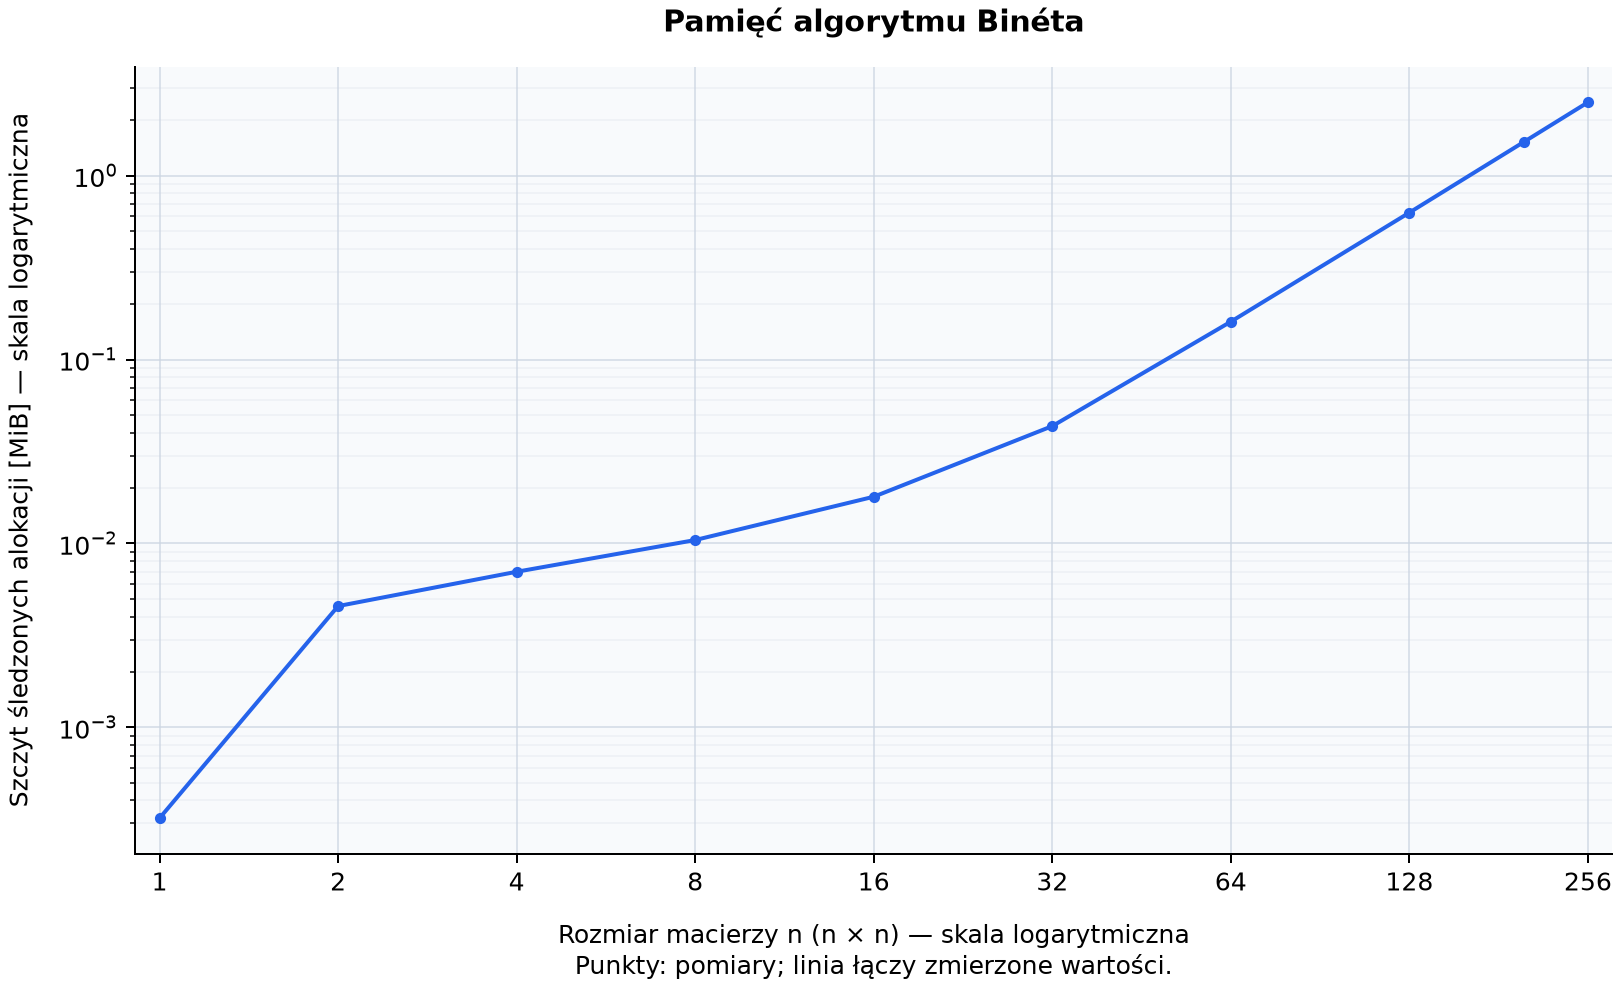
\includegraphics[width=0.9\linewidth]{assets/binet_memory.png}
    \label{fig:placeholder}
\end{figure}

\begin{table}[htpb]
\centering
\caption{Wyniki czasowe i operacyjne (metoda Bineta)}
\label{tab:binet_results}
\begin{tabular}{r | r r r r}
\toprule
Rozmiar $n$ & Czas [s] & Mnożenia & Dodawania & FLOPy \\
\midrule
1 & 0.000001 & 1 & 0 & 1 \\
2 & 0.000047 & 8 & 4 & 12 \\
4 & 0.000205 & 64 & 48 & 112 \\
8 & 0.001668 & 512 & 448 & 960 \\
16 & 0.012699 & 4096 & 3840 & 7936 \\
32 & 0.117137 & 32768 & 31744 & 64512 \\
64 & 0.980779 & 262144 & 258048 & 520192 \\
128 & 7.080032 & 2097152 & 2080768 & 4177920 \\
200 & 17.443452 & 8000000 & 7960000 & 15960000 \\
256 & 56.590433 & 16777216 & 16711680 & 33488896 \\
512 & 429.223804 & 134217728 & 133955584 & 268173312 \\
\bottomrule
\end{tabular}
\end{table}

\begin{figure}
    \centering
    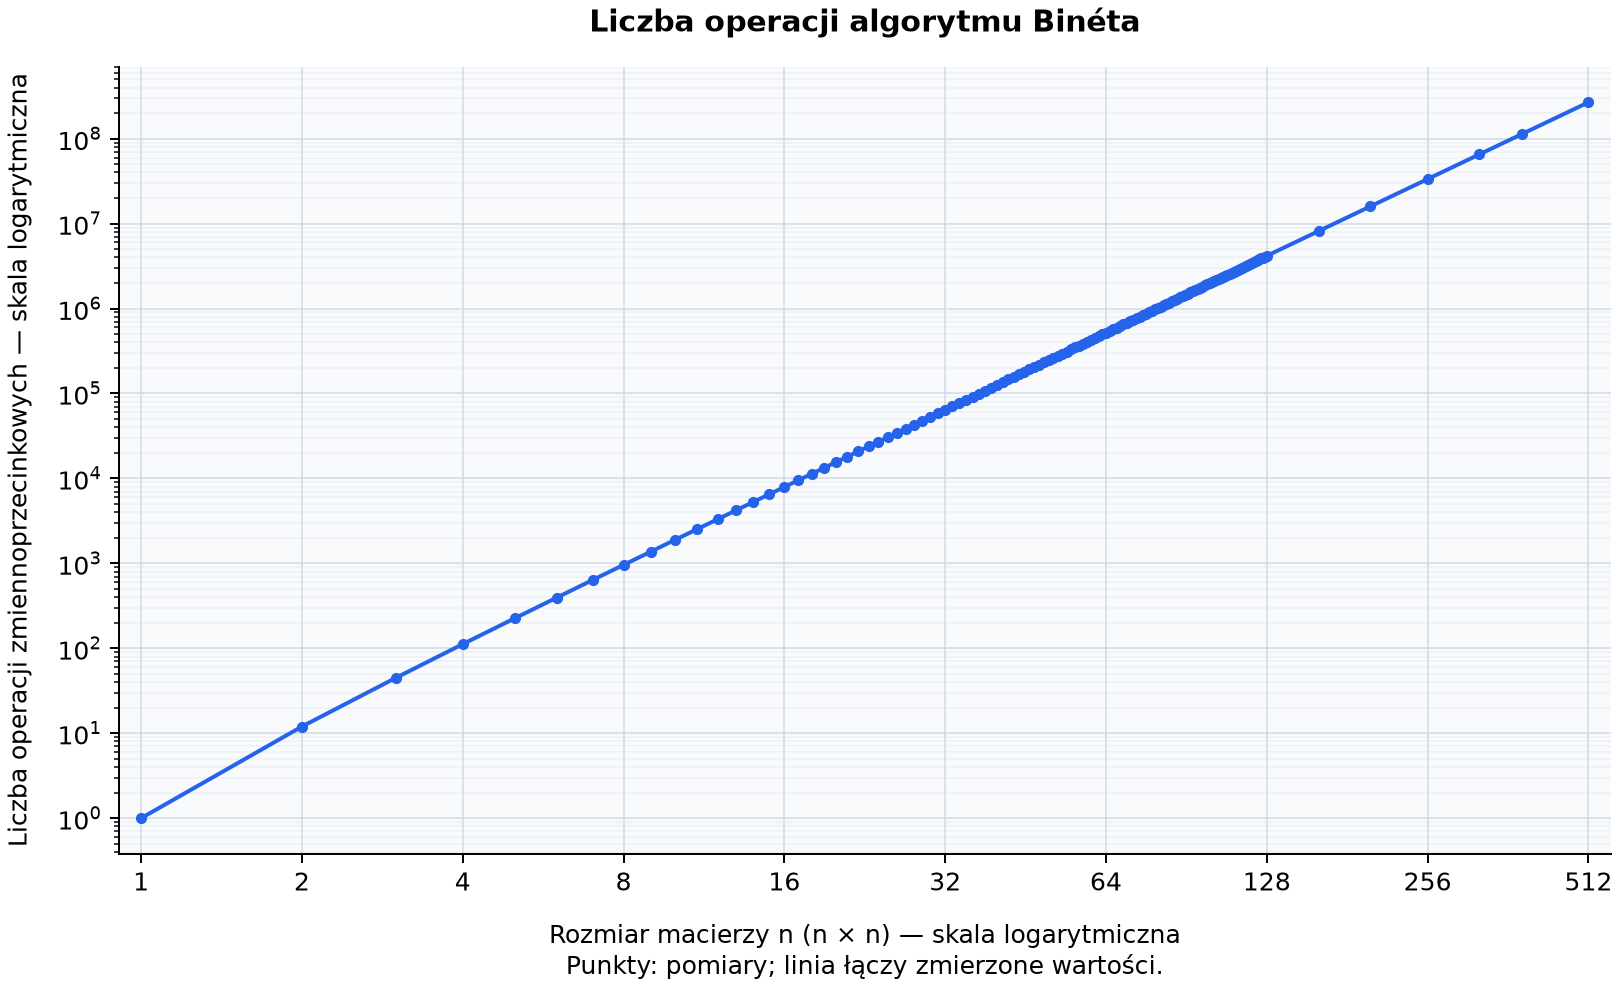
\includegraphics[width=0.9\linewidth]{assets/binet_flops.png}
    \label{fig:placeholder}
\end{figure}

\begin{figure}
    \centering
    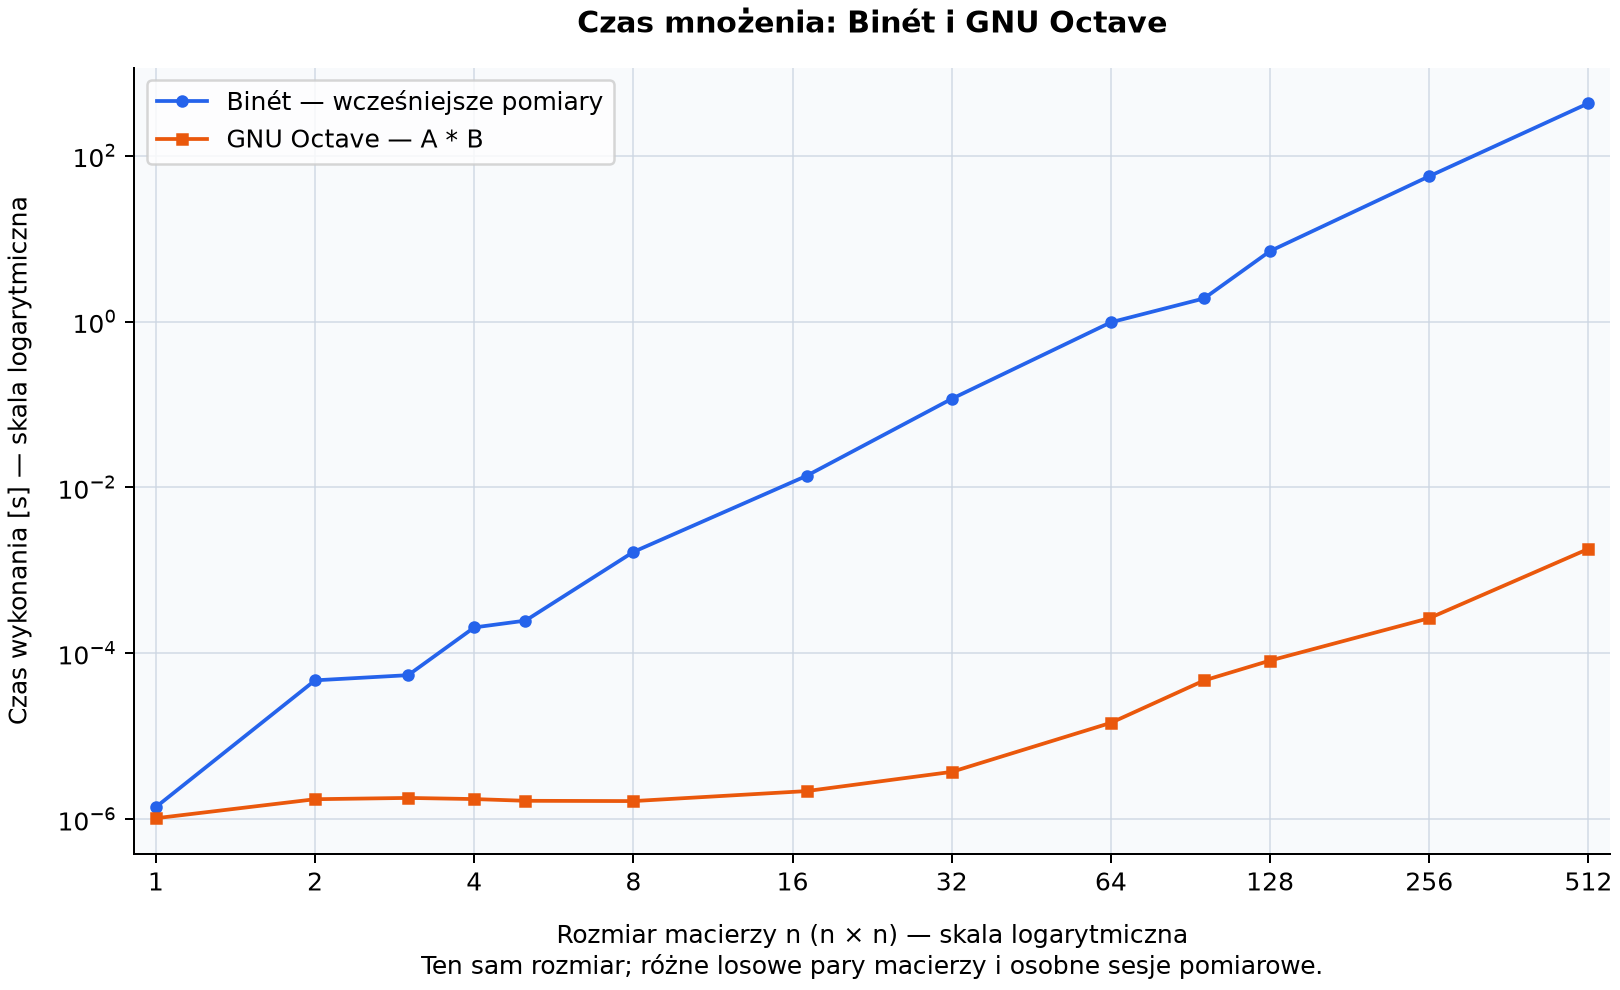
\includegraphics[width=0.9\linewidth]{assets/binet_octave_time.png}
    \label{fig:placeholder}
\end{figure}

\newpage

\section{Algorytm Strassena}

Kolejnym rozważanym algorytmem jest metoda Strassena, która stanowi asymptotycznie szybszą alternatywę dla klasycznego mnożenia blokowego. Podobnie jak w metodzie Bineta, algorytm ten opiera się na strategii ,,dziel i zwyciężaj'', w której macierze wejściowe $A$ i $B$ o rozmiarach $n \times n$ dzielone są na cztery submacierze o wymiarach $\frac{n}{2} \times \frac{n}{2}$.

Kluczową innowacją tej metody jest redukcja liczby wywołań rekurencyjnych z $8$ do $7$. Pozwala to na obniżenie złożoności obliczeniowej z $\mathcal{O}(n^3)$ do $\mathcal{O}(n^{\log_2 7}) \approx \mathcal{O}(n^{2.81})$.

\[
\renewcommand{\arraystretch}{1.5}
C = \begin{pmatrix} 
P_1 + P_4 - P_5 + P_7 & P_3 + P_5 \\ 
P_2 + P_4 & P_1 - P_2 + P_3 + P_6 
\end{pmatrix}
\]

W dalszej części sprawozdania zbadamy wydajność czasową oraz pamięciową tego algorytmu w zależności od rozmiaru macierzy, a następnie zestawimy uzyskane wyniki z klasyczną metodą Bineta, aby sprawdzić, kiedy teoretyczny zysk wydajnościowy rekompensuje większy narzut operacyjny.

\begin{center}
\renewcommand{\arraystretch}{1.5}
\begin{tabular}{|l|}
\hline
$[C, \text{mul}, \text{add}] = \text{Strassen}(A, B)$ \\
\hline
\\
\textbf{\textcolor{blue}{if}} $n = 1$ \\
\quad \textcolor{red}{\rule{14cm}{0.6pt}} \\
\quad $\begin{aligned}
    C &:= \begin{pmatrix} A_{0,0} \cdot B_{0,0} \end{pmatrix} \\
    \text{mul} &:= 1 \\
    \text{add} &:= 0
\end{aligned}$ \\
\quad \textcolor{red}{\rule{14cm}{0.6pt}} \\
\\
\textbf{\textcolor{blue}{else if}} $n \pmod 2 = 1$ \\
\quad \textcolor{red}{\rule{14cm}{0.6pt}} \\
\quad $[C, \text{mul}, \text{add}] := \text{StrassenOdd}(A, B)$ \\
\quad \textcolor{red}{\rule{14cm}{0.6pt}} \\
\\
\textbf{\textcolor{blue}{else}} \\
\quad $A \rightarrow \left( \begin{array}{c|c}
    A_{11} & A_{12} \\ \hline
    A_{21} & A_{22}
\end{array} \right), \quad
B \rightarrow \left( \begin{array}{c|c}
    B_{11} & B_{12} \\ \hline
    B_{21} & B_{22}
\end{array} \right)$ \\
\\
\quad \textcolor{red}{\rule{14cm}{0.6pt}} \\
\quad $\begin{aligned}
    {[}P_1, m_1, a_1{]} &:= \text{Strassen}(A_{11} + A_{22}, B_{11} + B_{22}) \\
    {[}P_2, m_2, a_2{]} &:= \text{Strassen}(A_{21} + A_{22}, B_{11}) \\
    {[}P_3, m_3, a_3{]} &:= \text{Strassen}(A_{11}, B_{12} - B_{22}) \\
    {[}P_4, m_4, a_4{]} &:= \text{Strassen}(A_{22}, B_{21} - B_{11}) \\
    {[}P_5, m_5, a_5{]} &:= \text{Strassen}(A_{11} + A_{12}, B_{22}) \\
    {[}P_6, m_6, a_6{]} &:= \text{Strassen}(A_{21} - A_{11}, B_{11} + B_{12}) \\
    {[}P_7, m_7, a_7{]} &:= \text{Strassen}(A_{12} - A_{22}, B_{21} + B_{22}) \\
    C_{11} &:= P_1 + P_4 - P_5 + P_7 \\
    C_{12} &:= P_3 + P_5 \\
    C_{21} &:= P_2 + P_4 \\
    C_{22} &:= P_1 - P_2 + P_3 + P_6 \\
    \text{mul} &:= \sum_{i=1}^{7} m_i \\
    \text{add} &:= \sum_{i=1}^{7} a_i + 18 \cdot \left(\frac{n}{2}\right)^2
\end{aligned}$ \\
\quad \textcolor{red}{\rule{14cm}{0.6pt}} \\
\\
\quad $C \leftarrow \left( \begin{array}{c|c}
    C_{11} & C_{12} \\ \hline
    C_{21} & C_{22}
\end{array} \right)$ \\
\\
\textbf{\textcolor{blue}{endif}} \\
\hline
\end{tabular}
\end{center}

\newpage

\subsection{Rozszerzenie metody Strassena na dowolne rozmiary macierzy kwadratowych}

Wzory Strassena wymagają bloków o jednakowych rozmiarach, ponieważ dodajemy i odejmujemy bloki wejściowe jeszcze przed ich mnożeniem. Dla parzystego $n$ dzielimy zatem macierze na cztery równe części. Dla nieparzystego $n>1$ oddzielamy ostatni wiersz oraz ostatnią kolumnę, zamiast dopełniać macierze zerami:
\[
A=\begin{pmatrix} A_0 & a \\ r & \alpha \end{pmatrix},\qquad
B=\begin{pmatrix} B_0 & b \\ s & \beta \end{pmatrix}.
\]

Macierze $A_0$ i $B_0$ mają parzysty rozmiar $(n-1)\times(n-1)$. Symbole $a$ i $b$ oznaczają ostatnie kolumny bez dolnego elementu, $r$ i $s$ ostatnie wiersze bez prawego elementu, a $\alpha$ i $\beta$ elementy w prawym dolnym rogu. Iloczyn wyznaczamy ze wzoru
\[
AB=\begin{pmatrix}
\operatorname{Strassen}(A_0,B_0)+as & A_0b+a\beta \\
rB_0+\alpha s & rb+\alpha\beta
\end{pmatrix}.
\]

Główny iloczyn $A_0B_0$ obliczamy rekurencyjnie metodą Strassena. Pozostałe iloczyny, zawierające wektory lub skalary, wykonujemy funkcją \texttt{MultiplyDirect}, a następnie składamy cztery bloki wyniku. Przykładowo dla rozmiaru $5\times5$ część główna ma rozmiar $4\times4$, a pozostałe obliczenia dotyczą wydzielonego wiersza i kolumny.

Tę samą regułę stosujemy na każdym poziomie rekurencji, aż do przypadku $n=1$. W ten sposób algorytm obsługuje wszystkie dodatnie rozmiary macierzy kwadratowych, nie tylko potęgi dwójki. Obliczenia dotyczące wydzielonego brzegu mają koszt $\mathcal{O}(n^2)$, więc nie zmieniają dominującej złożoności $\mathcal{O}(n^{\log_2 7})$.

\begin{center}
\renewcommand{\arraystretch}{1.5}
\begin{tabular}{|l|}
\hline
$[C, \text{mul}, \text{add}] = \text{StrassenOdd}(A, B)$ \\
\hline
\\
$A \rightarrow \left( \begin{array}{c|c}
    A_0 & a \\ \hline
    r & \alpha
\end{array} \right), \quad
B \rightarrow \left( \begin{array}{c|c}
    B_0 & b \\ \hline
    s & \beta
\end{array} \right)$ \\
\\
\textcolor{red}{\rule{14cm}{0.6pt}} \\
$\begin{aligned}
    {[}P_1, m_1, a_1{]} &:= \text{Strassen}(A_0, B_0) \\
    {[}P_2, m_2, a_2{]} &:= \text{MultiplyDirect}(a, s) \\
    {[}P_3, m_3, a_3{]} &:= \text{MultiplyDirect}(A_0, b) \\
    {[}P_4, m_4, a_4{]} &:= \text{MultiplyDirect}(a, \beta) \\
    {[}P_5, m_5, a_5{]} &:= \text{MultiplyDirect}(r, B_0) \\
    {[}P_6, m_6, a_6{]} &:= \text{MultiplyDirect}(\alpha, s) \\
    {[}P_7, m_7, a_7{]} &:= \text{MultiplyDirect}(r, b) \\
    {[}P_8, m_8, a_8{]} &:= \text{MultiplyDirect}(\alpha, \beta) \\
    C_{11} &:= P_1 + P_2 \\
    C_{12} &:= P_3 + P_4 \\
    C_{21} &:= P_5 + P_6 \\
    C_{22} &:= P_7 + P_8 \\
    \text{mul} &:= \sum_{i=1}^{8} m_i \\
    \text{add} &:= \sum_{i=1}^{8} a_i + \text{size}(C_{11}) + \text{size}(C_{12}) + \text{size}(C_{21}) + \text{size}(C_{22})
\end{aligned}$ \\
\textcolor{red}{\rule{14cm}{0.6pt}} \\
\\
$C \leftarrow \left( \begin{array}{c|c}
    C_{11} & C_{12} \\ \hline
    C_{21} & C_{22}
\end{array} \right)$ \\
\\
\hline
\end{tabular}
\end{center}

\begin{table}[htpb]
\centering
\caption{Wyniki zużycia pamięci (metoda Strassena)}
\label{tab:strassen_memory}
\begin{tabular}{r | r r r r r}
\toprule
Rozmiar $n$ & Pamięć szczyt. [MiB] & Pamięć wej. [MiB] & Mnożenia & Dodawania & FLOPy \\
\midrule
1 & 0.000420 & 0.000015 & 1 & 0 & 1 \\
2 & 0.004463 & 0.000061 & 7 & 18 & 25 \\
4 & 0.006607 & 0.000244 & 49 & 198 & 247 \\
8 & 0.009537 & 0.000977 & 343 & 1674 & 2017 \\
16 & 0.015762 & 0.003906 & 2401 & 12870 & 15271 \\
32 & 0.041237 & 0.015625 & 16807 & 94698 & 111505 \\
64 & 0.152565 & 0.062500 & 117649 & 681318 & 798967 \\
128 & 0.597878 & 0.250000 & 823543 & 4842954 & 5666497 \\
200 & 1.453865 & 0.610352 & 3676617 & 10579592 & 14256209 \\
256 & 2.379128 & 1.000000 & 5764801 & 34195590 & 39960391 \\
\bottomrule
\end{tabular}
\end{table}

\begin{figure}
    \centering
    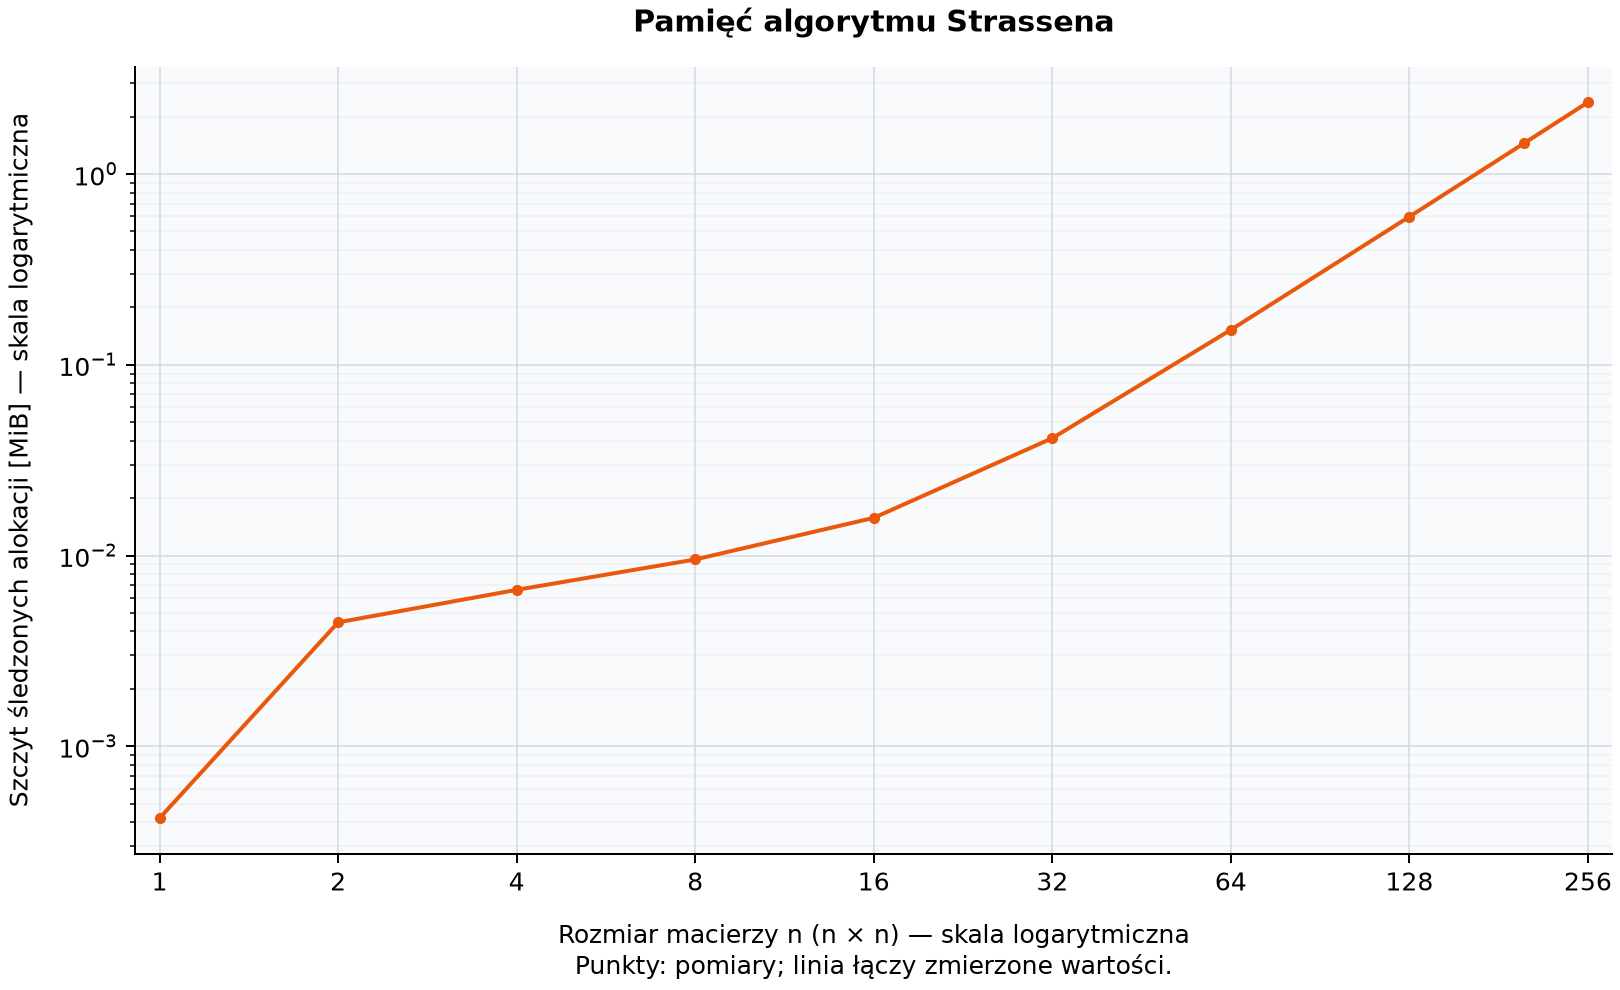
\includegraphics[width=0.9\linewidth]{assets/strassen_memory.png}
    \label{fig:strassen_memory_plot}
\end{figure}

\begin{table}[htpb]
\centering
\caption{Wyniki czasowe i operacyjne (metoda Strassena)}
\label{tab:strassen_results}
\begin{tabular}{r | r r r r}
\toprule
Rozmiar $n$ & Czas [s] & Mnożenia & Dodawania & FLOPy \\
\midrule
1 & 0.000002 & 1 & 0 & 1 \\
2 & 0.000034 & 7 & 18 & 25 \\
3 & 0.000061 & 26 & 32 & 58 \\
4 & 0.000226 & 49 & 198 & 247 \\
5 & 0.000271 & 110 & 250 & 360 \\
8 & 0.001624 & 343 & 1674 & 2017 \\
17 & 0.012249 & 3218 & 13654 & 16872 \\
32 & 0.083366 & 16807 & 94698 & 111505 \\
64 & 0.584557 & 117649 & 681318 & 798967 \\
96 & 1.044563 & 436982 & 1390106 & 1827088 \\
128 & 4.023335 & 823543 & 4842954 & 5666497 \\
256 & 29.379938 & 5764801 & 34195590 & 39960391 \\
512 & 210.828233 & 40353607 & 240548778 & 280902385 \\
\bottomrule
\end{tabular}
\end{table}

\begin{figure}
    \centering
    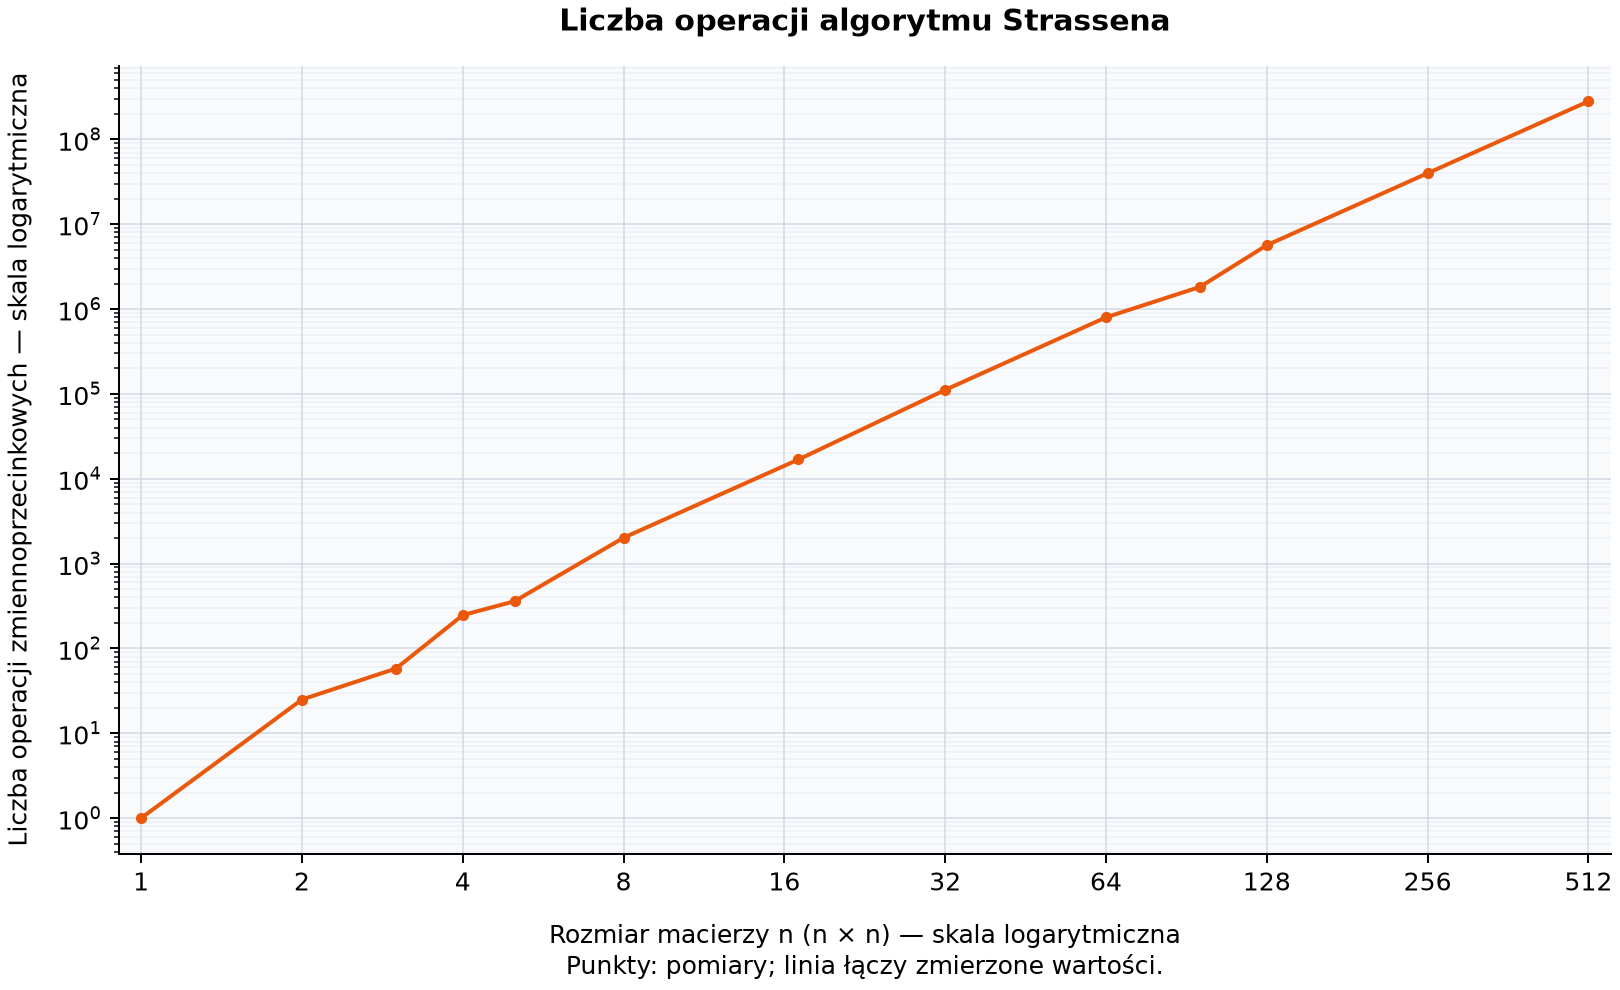
\includegraphics[width=0.9\linewidth]{assets/strassen_flops.png}
    \label{fig:strassen_flops_plot}
\end{figure}

\newpage

\section{Algorytm AlphaTensor}
Kolejnym rozważanym algorytmem jest metoda oparta na algorytmach odkrytych przez system AlphaTensor, która stanowi nowoczesną, wygenerowaną przez sztuczną inteligencję alternatywę dla klasycznego mnożenia blokowego. Podobnie jak w poprzednich metodach, algorytm ten opiera się na strategii ,,dziel i zwyciężaj'', w której macierze wejściowe są dzielone na mniejsze podmacierze.

\begin{center}
\renewcommand{\arraystretch}{1.5}
\begin{tabular}{|l|}
\hline
$[C, \text{mul}, \text{add}] = \text{AlphaTensor}(A, B)$ \\
\hline
\\
\textbf{\textcolor{blue}{if}} $\text{rows}(A) < 4$ \textbf{or} $\text{cols}(A) < 5$ \textbf{or} $\text{cols}(B) < 5$ \\
\quad \textcolor{red}{\rule{14cm}{0.6pt}} \\
\quad $[C, \text{mul}, \text{add}] := \text{MultiplyDirect}(A, B)$ \\
\quad \textcolor{red}{\rule{14cm}{0.6pt}} \\
\\
\textbf{\textcolor{blue}{else}} \\
\quad $\begin{aligned}
    \tilde{A} &:= \text{Pad}(A, 4, 5) \quad \text{(pad to sizes divisible by 4 and 5)} \\
    \tilde{B} &:= \text{Pad}(B, 5, 5) \quad \text{(pad to sizes divisible by 5)}
\end{aligned}$ \\
\quad $\tilde{A} \rightarrow \left( A_{i,j} \right)_{\substack{0 \le i < 4 \\ 0 \le j < 5}}, \quad
\tilde{B} \rightarrow \left( B_{j,k} \right)_{\substack{0 \le j < 5 \\ 0 \le k < 5}}$ \\
\\
\quad \textcolor{red}{\rule{14cm}{0.6pt}} \\
\quad \textbf{\textcolor{blue}{for}} $r = 0$ \textbf{\textcolor{blue}{to}} $\text{size}(U) - 1$ \textbf{\textcolor{blue}{do}} \\
\quad $\begin{aligned}
    [L_r, \text{op}_{L,r}] &:= \text{Combine}( \{A_{i,j}\}, U_r ) \\
    [R_r, \text{op}_{R,r}] &:= \text{Combine}( \{B_{j,k}\}, V_r ) \\
    [P_r, m_r, a_r] &:= \text{AlphaTensor}(L_r, R_r)
\end{aligned}$ \\
\quad \textbf{\textcolor{blue}{endfor}} \\
\\
\quad \textbf{\textcolor{blue}{for}} $idx = 0$ \textbf{\textcolor{blue}{to}} $19$ \textbf{\textcolor{blue}{do}} \\
\quad $\begin{aligned}
    i &:= \lfloor idx / 5 \rfloor, \quad k := idx \pmod 5 \\
    [C_{i,k}, \text{op}_{C,idx}] &:= \text{Combine}( \{P_r\}, W_{idx} )
\end{aligned}$ \\
\quad \textbf{\textcolor{blue}{endfor}} \\
\\
\quad $\begin{aligned}
    \text{mul} &:= \sum m_r \\
    \text{add} &:= \sum a_r + \sum \text{op}_{L,r} + \sum \text{op}_{R,r} + \sum \text{op}_{C,idx}
\end{aligned}$ \\
\quad \textcolor{red}{\rule{14cm}{0.6pt}} \\
\\
\quad $\tilde{C} \leftarrow \left( \begin{array}{ccc} C_{0,0} & \cdots & C_{0,4} \\ \vdots & \ddots & \vdots \\ C_{3,0} & \cdots & C_{3,4} \end{array} \right)$ \\
\quad $C \leftarrow \tilde{C}[0:\text{rows}(A), 0:\text{cols}(B)]$ \\
\\
\textbf{\textcolor{blue}{endif}} \\
\hline
\end{tabular}
\end{center}

\begin{table}[htpb]
\centering
\caption{Wyniki zużycia pamięci (metoda AlphaTensor)}
\label{tab:alphatensor_memory}
\begin{tabular}{r | r r r r r}
\toprule
Rozmiar $n$ & Pamięć szczyt. [MiB] & Pamięć wej. [MiB] & Mnożenia & Dodawania & FLOPy \\
\midrule
1 & 0.000290 & 0.000015 & 1 & 0 & 1 \\
2 & 0.000412 & 0.000061 & 8 & 4 & 12 \\
4 & 0.000504 & 0.000244 & 64 & 48 & 112 \\
8 & 0.022034 & 0.000977 & 608 & 2500 & 3108 \\
16 & 0.035309 & 0.003906 & 4864 & 12432 & 17296 \\
32 & 0.112282 & 0.015625 & 46208 & 219386 & 265594 \\
64 & 0.272316 & 0.062500 & 207936 & 701706 & 909642 \\
128 & 1.004868 & 0.250000 & 3511808 & 16692328 & 20204136 \\
200 & 1.611801 & 0.610352 & 7023616 & 29167760 & 36191376 \\
256 & 3.748520 & 1.000000 & 15803136 & 53464600 & 69267736 \\
\bottomrule
\end{tabular}
\end{table}

\begin{figure}
    \centering
    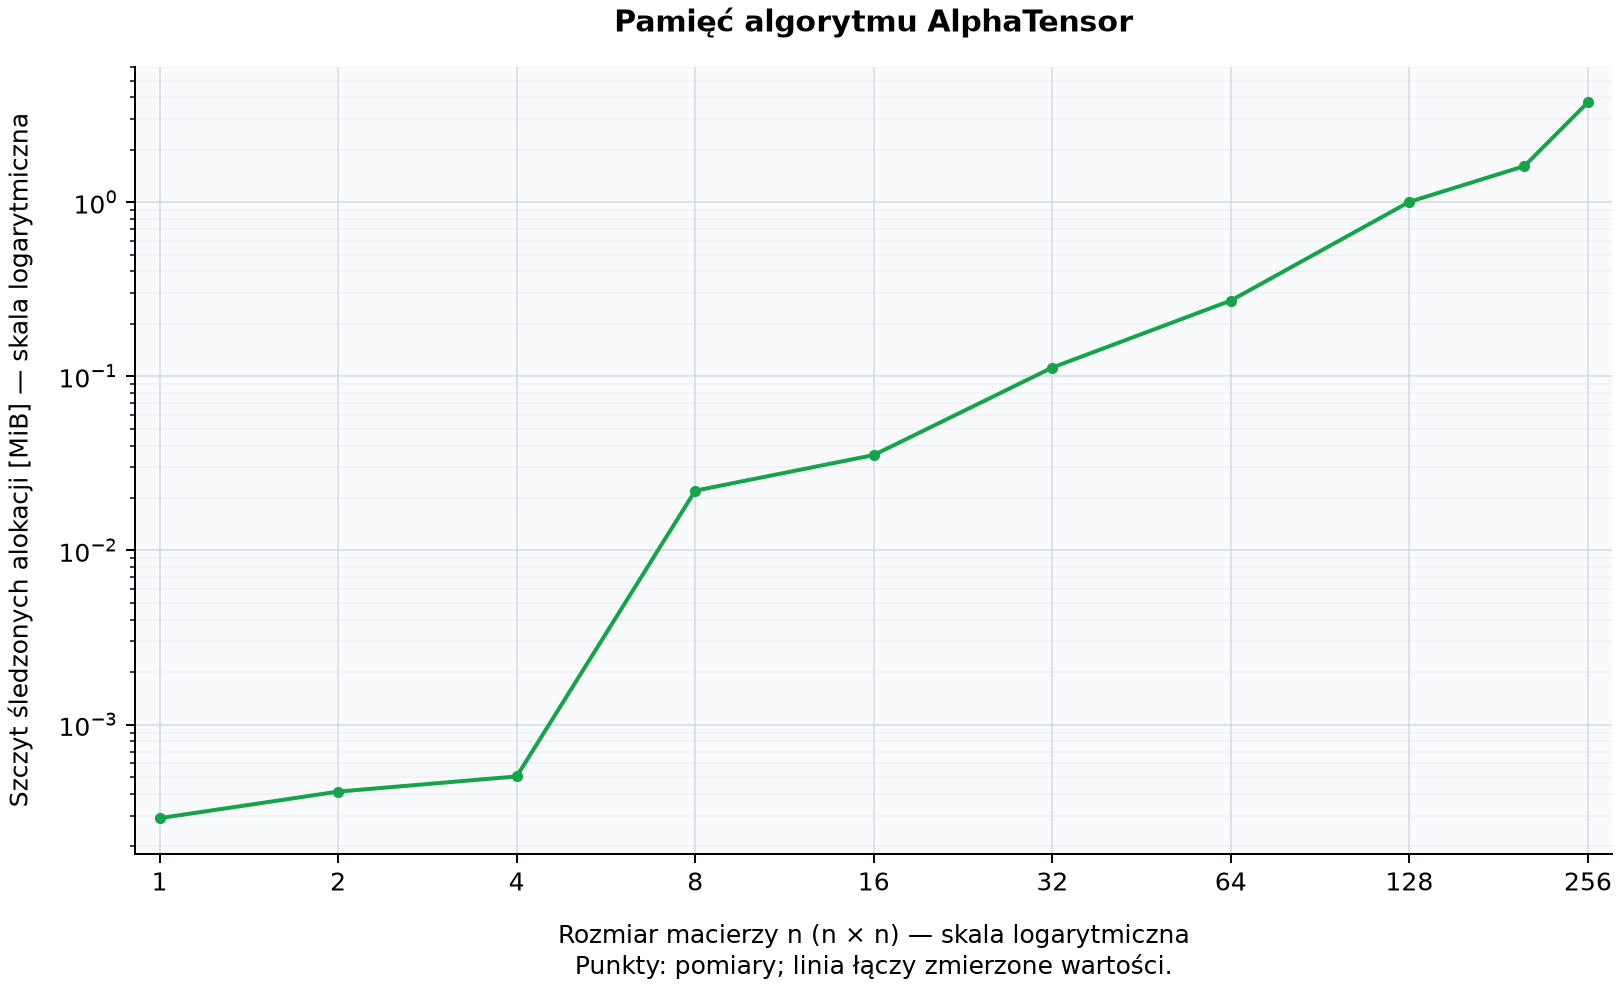
\includegraphics[width=0.9\linewidth]{assets/alphatensor_memory.png}
    \label{fig:alphatensor_memory_plot}
\end{figure}

\begin{table}[htpb]
\centering
\caption{Wyniki czasowe i operacyjne (metoda AlphaTensor)}
\label{tab:alphatensor_results}
\begin{tabular}{r | r r r r}
\toprule
Rozmiar $n$ & Czas [s] & Mnożenia & Dodawania & FLOPy \\
\midrule
1 & 0.000002 & 1 & 0 & 1 \\
2 & 0.000004 & 8 & 4 & 12 \\
3 & 0.000012 & 27 & 18 & 45 \\
4 & 0.000024 & 64 & 48 & 112 \\
5 & 0.000729 & 152 & 904 & 1056 \\
8 & 0.001145 & 608 & 2500 & 3108 \\
17 & 0.003243 & 6080 & 14764 & 20844 \\
32 & 0.082191 & 46208 & 219386 & 265594 \\
64 & 0.151042 & 207936 & 701706 & 909642 \\
96 & 0.281255 & 554496 & 1547296 & 2101792 \\
128 & 6.711583 & 3511808 & 16692328 & 20204136 \\
256 & 12.819688 & 15803136 & 53464600 & 69267736 \\
512 & 357.719349 & 66724352 & 538238234 & 604962586 \\
\bottomrule
\end{tabular}
\end{table}

\begin{figure}
    \centering
    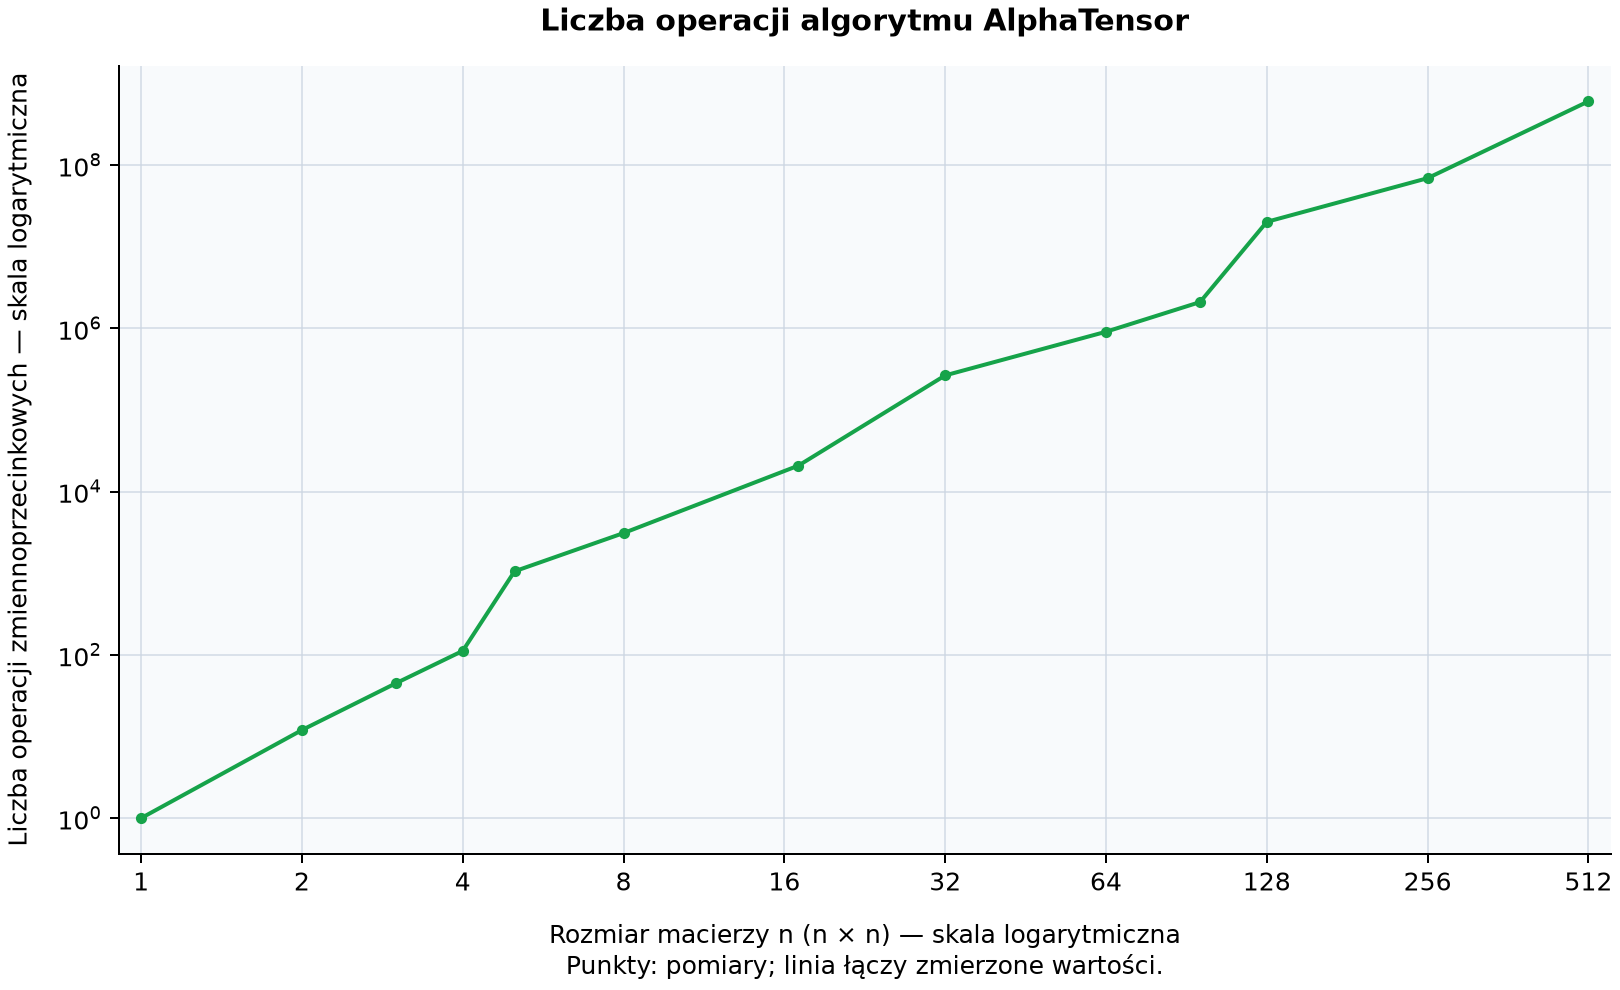
\includegraphics[width=0.9\linewidth]{assets/alphatensor_flops.png}
    \label{fig:alphatensor_flops_plot}
\end{figure}

\newpage

\section{Porównanie wyników}

\begin{figure}[H]
    \centering
    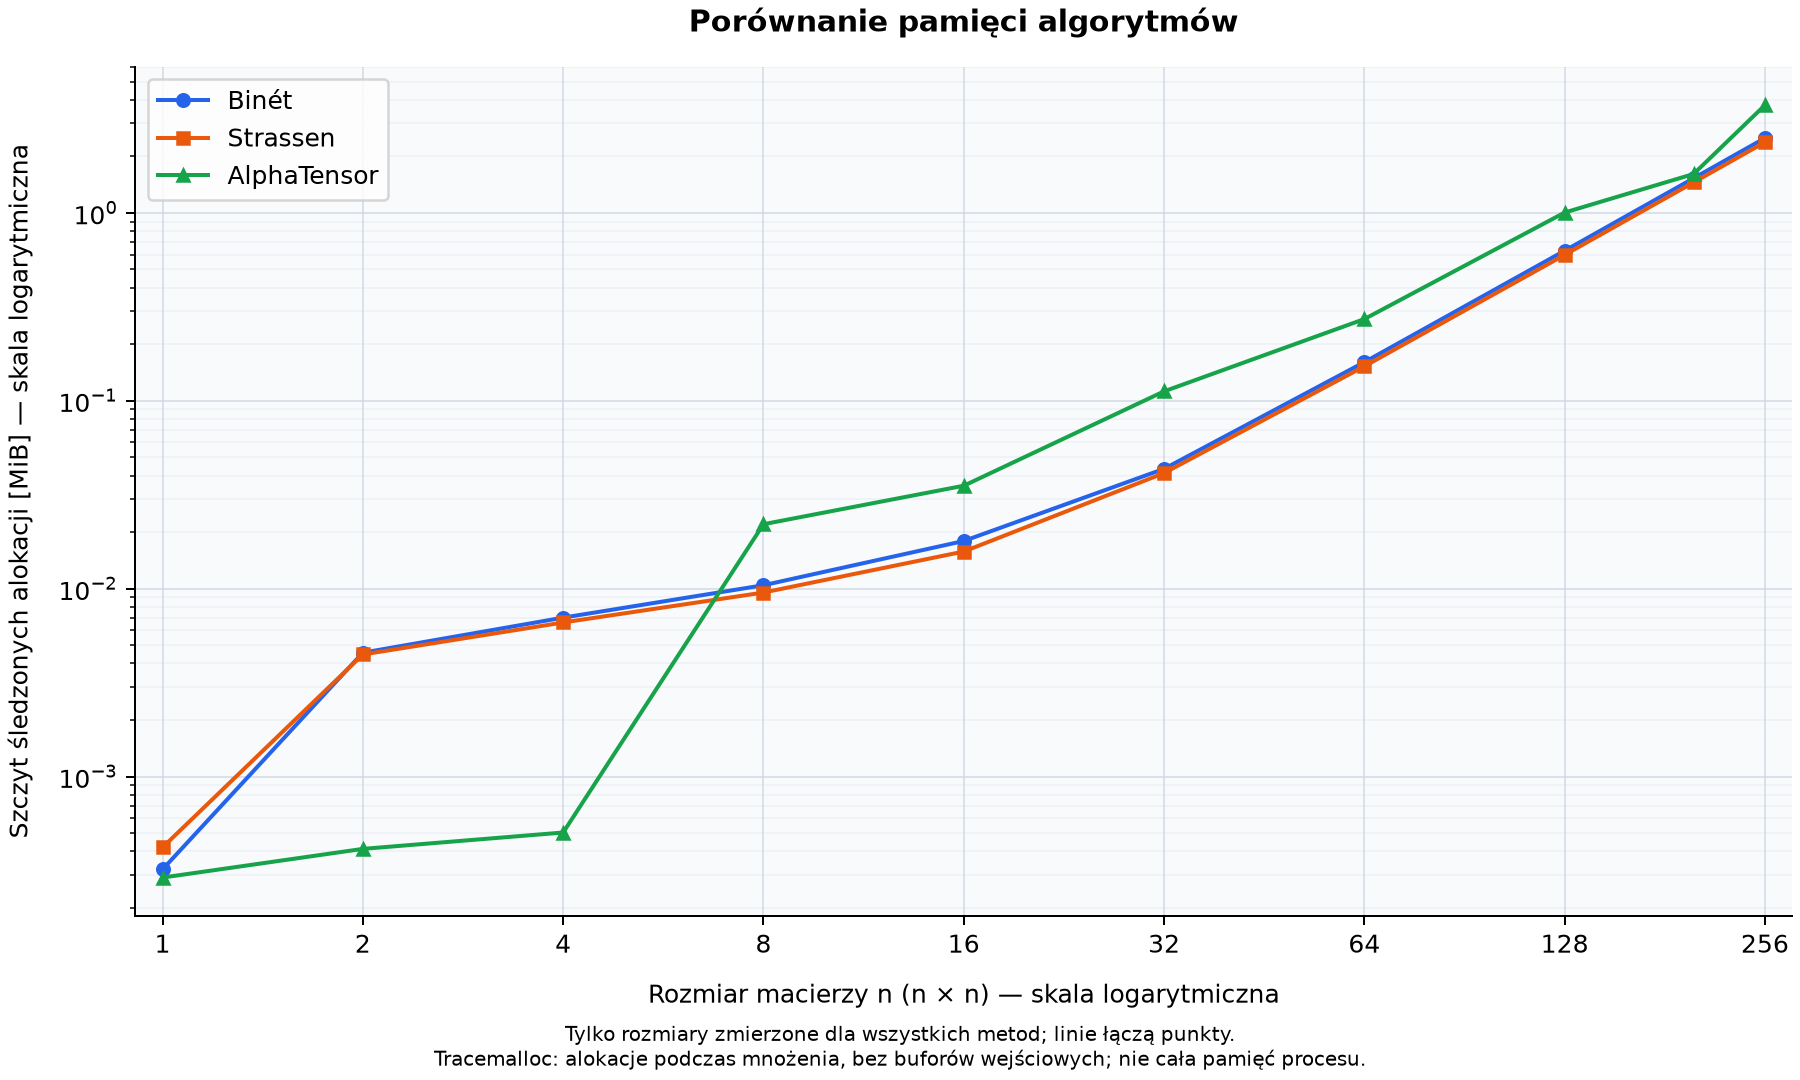
\includegraphics[width=0.9\linewidth]{assets/comparison_memory.png}
    \label{fig:placeholder}
\end{figure}

\begin{figure}[H]
    \centering
    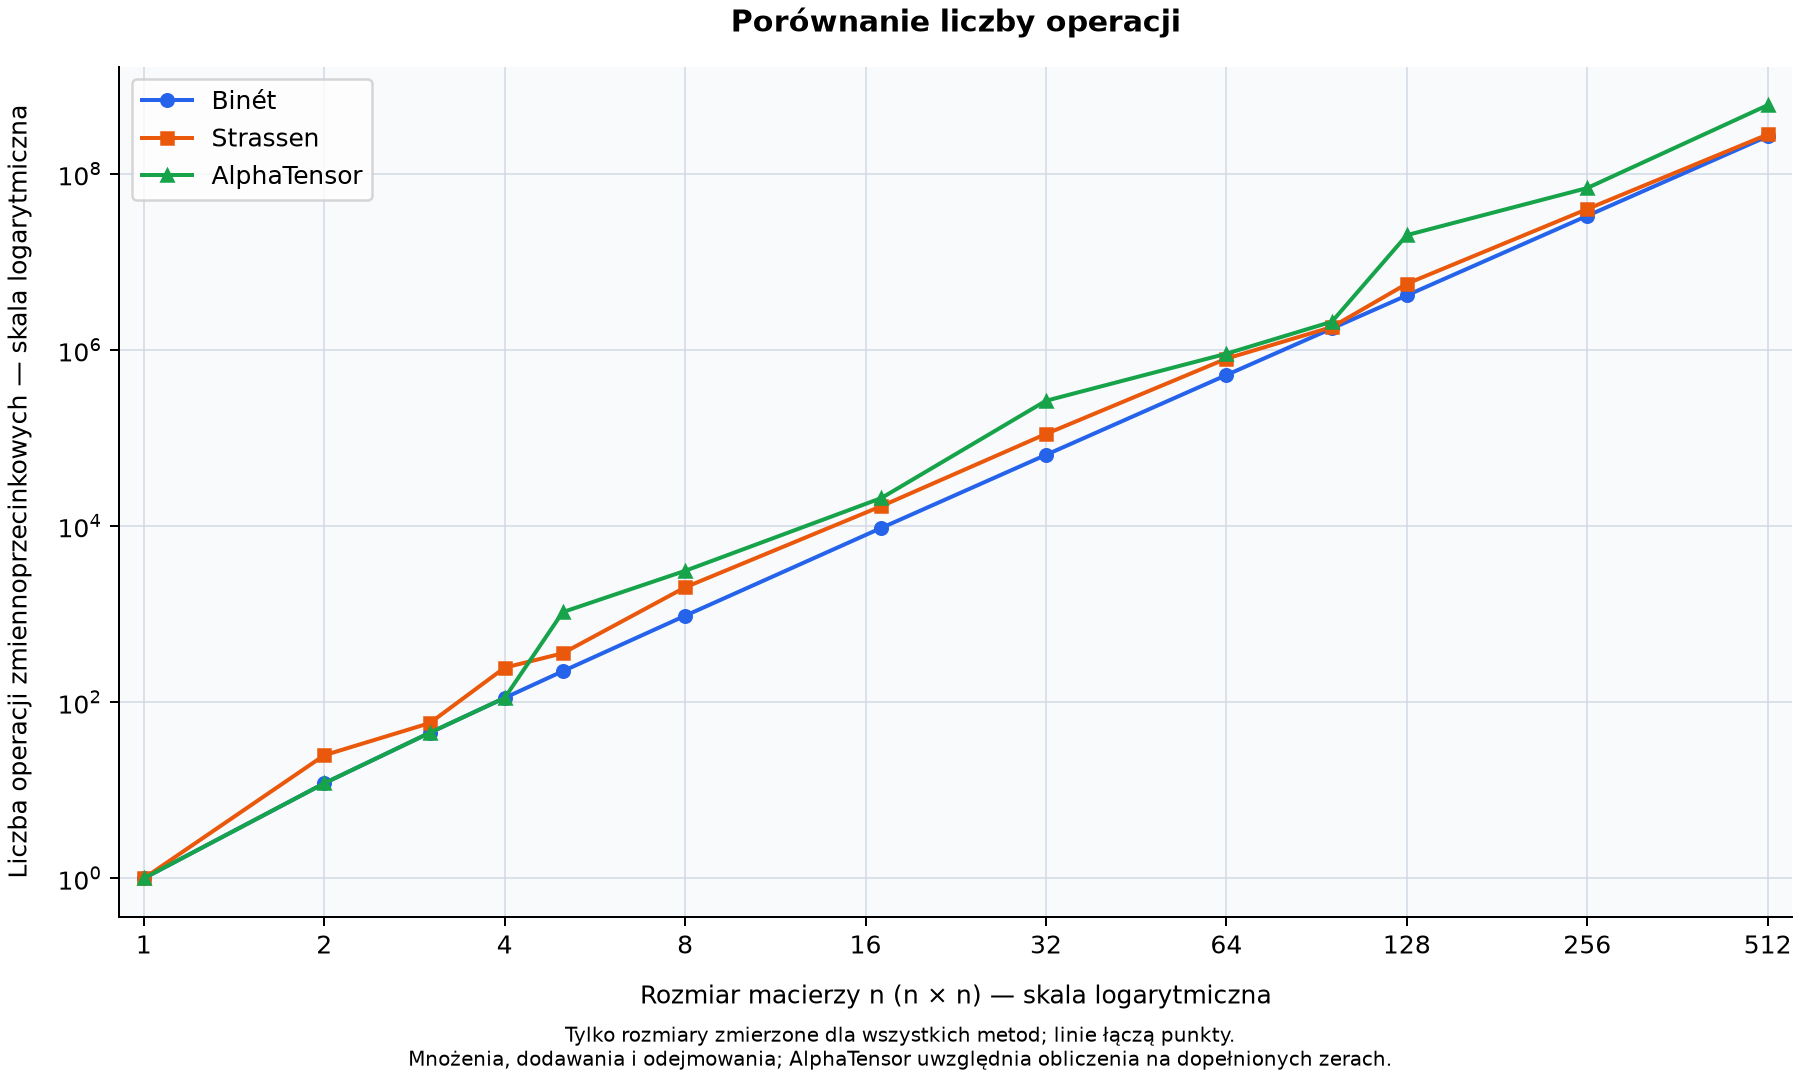
\includegraphics[width=0.9\linewidth]{assets/comparison_flops.png}
    \label{fig:placeholder}
\end{figure}


\begin{figure}[H]
    \centering
    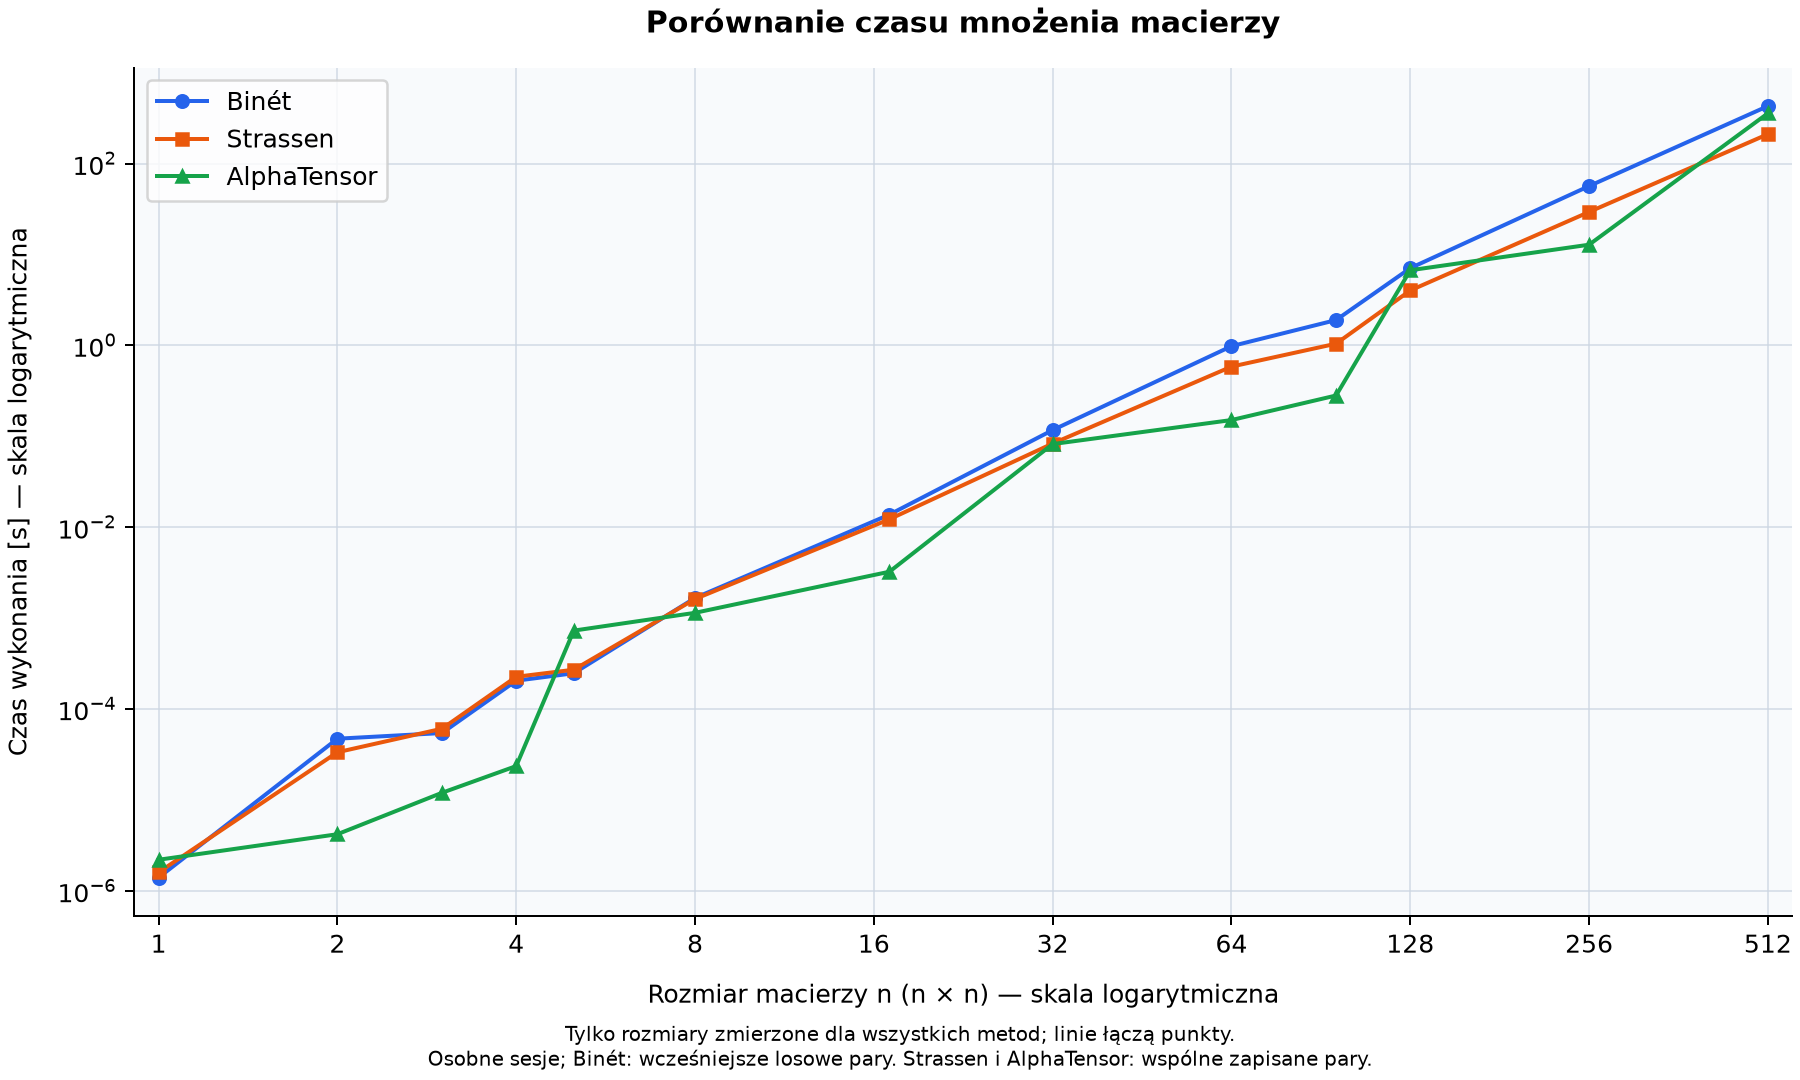
\includegraphics[width=0.9\linewidth]{assets/comparison_time.png}
    \label{fig:placeholder}
\end{figure}


\printbibliography[title={Literatura}]

\end{document}